\documentclass[conference]{IEEEtran}
\IEEEoverridecommandlockouts
% The preceding line is only needed to identify funding in the first footnote. If that is unneeded, please comment it out.
\usepackage{soul}
\usepackage{amssymb,amsmath,bm}
\usepackage{graphics,adjustbox}
\usepackage{tikz}
\usepackage{subfigure}
\usepackage{epstopdf}
\epstopdfsetup{suffix={}}
\usepackage{siunitx}
\sisetup{unitsep = \cdot}

\usepackage[figuresright]{rotating}
\usepackage[colorinlistoftodos]{todonotes}
\usepackage[english,algo2e,algoruled,vlined,linesnumbered]{algorithm2e}   % package for algorithm
\usepackage{enumerate}

\usepackage{easyReview}
\newtheorem{assumption}{Assumption}


\DeclareMathOperator*{\argmin}{arg min}

\def\BibTeX{{\rm B\kern-.05em{\sc i\kern-.025em b}\kern-.08em
    T\kern-.1667em\lower.7ex\hbox{E}\kern-.125emX}}
\begin{document}

\title{A Novel Model-Free Learning Approach for Dynamic Target Tracking Problem and its Validation using Virtual Robot Experimentation Platform 
%  
% \thanks{This work was supported in part by the Bradley University’s Caterpillar fellowship grant.}
}

\author{%~
\IEEEauthorblockN{Amr Elhussein and Md Suruz Miah}
\IEEEauthorblockA{\textit{Electrical \& Computer Eng.} \\
\textit{Bradley University}, Peoria, Illinois, USA \\
 aelhussein@mail.bradley.edu and smiah@bradley.edu}
% \and
% \IEEEauthorblockN{Fazel Keshtkar}
% \IEEEauthorblockA{\textit{Div. of Computer Science, Math. and Science} \\
% \textit{St John's University}, Queens, NY, USA \\
% keshtkaf@stjohns.edu}
% \and
% \IEEEauthorblockN{Mohammed Abouheaf}
% \IEEEauthorblockA{\textit{School of EECS} \\
% \textit{Univ. of Ottawa}, Canada\\
% mabouhea@uottawa.ca}
%
}

\maketitle

\begin{abstract}
  %
  Addressing the trajectory tracking problem of a mobile robot in tracking a dynamic target is still one of the challenging problems in the field of robotics. In this paper, we address the position tracking problem of a mobile robot where it is supposed to track the position of an mobile target whose dynamics is unknown a priori. This problem is even more challenging when the dynamics of the mobile robot is also assumed to be unknown, which is a basically a realistic assumption. Most of trajectory tracking problems proposed in the literature in the field of mobile robotics are either focused on algorithms that rely on mathematical models of the robots or driven by a  overwhelming degree of computational complexity. This paper proposes a model-free actor-critic reinforcement learning strategy to determine appropriate actuator commands for the robot to track the position trajectory (unknown a priori) of the target. We emphasize that mathematical models of both mobile robot and the target are not required in the current approach. Moreover, Bellman's principle of optimality is utilized to minimize the energy required for the robot to track the target. The performance of the proposed actor-critic reinforcement learning approach  is backed by a set of computer simulations with various complexities using a virtual circular-shaped mobile robot and a point target  modeled by an integrator. 

%   It is even more challenging 
% This paper advances the previous work done by authors by validating a model-free actor-critic reinforcement learning approach to solve dynamic target tracking problem for a car-like mobile robot. The learning approach generates the linear velocity and steering angle of the robot and it does not require any prior knowledge of the dynamic model of the moving target. Policy iteration approach is employed through Bellman's principle of optimality to assess the cost of the control actions derived by the proposed learning method. The algorithm is tested by coducting a set of computer expeeriments for complex secnarios using virtual robot expirementation platform widely known as CoppeliaSim.        
% }{Need to be rewritten}  
%
\end{abstract}

\begin{IEEEkeywords}
Leader-follower formation, mobile robots, reinforcement learning, policy iteration, trajectory tracking
\end{IEEEkeywords}

% \begin{nomenclature}
% \begin{deflist}[A]
% \defitem{ADP} \defterm{Approximate dynamic programming}
% \defitem{AL}\defterm{Approximate linearization}
% \defitem{RL}\defterm{Reinforcement learning}
% \end{deflist}
% \end{nomenclature}

\section{Introduction}
\label{sec:introduction}
\todo[inline]{Need to discuss in details the limitations of previous work, we
  can also add RL applications to robotics navigation}

Tracking a random moving target using a mobile robot, for instance, is a challenging task. This is mainly due to their inherent complex nonlinear dynamics. Most of the target tracking algorithms proposed in the literature either rely on A) complex mathematical models, B) simplified mathematical models, and C) nonlinear control techniques or driven by large amount of mostly offline data that leads to an overwhelming degree of computational complexity.


Over the past years mobile robots has been used in several applications in commercial and military sectors such as surveillance, search and rescue missions,coverage optimization, cooperative localization and dynamic target tracking tasks \cite{kolling2006},\cite{Encarnacao2001},\cite{Ju2001}.  In all of these mentioned applications a fleet of robot i.e agents interact with each other to achieve a certain goal. Leader-Follower or dynamic target tracking problem has recieved an extensive amount of study and research in the world of cooperative control theory due to it's wide promising applications such as search and rescure missions, wildlife monitoring and survillance to name a few . In a typical leader follower formation a number of robots referred to as followers apply local control actions to follow leader's robots in a specific predefined path such as \hl {cyclic, circular motion and time varying communication topologies.} \hl {limitations of other methods} many control methods were proposed however they have had the following limitations:
\\(1) a static leader/target is used.
\\(2) the leade/target's location or dynamic model is predetermined.  
\\(3) expensive hardware platforms are used to achieve the mobile target tracking. 

The main contribution of this work is the development of a model-free learning approach to control the follower robot by which it overcome many of the limitations mentiond above as it does not rely on any prior information of the mathmetical model or the dynamic model. The steering angle and the linear speed of the follower robot are determined by collecting the position and orientation of both the leader and the follower. This set of information is gathered online over a finite period of time. The optimal control actions are then generated by utilizing Bellman's principal of optimality which acts as model free-reinfocment learning approach that allows the follower robot to follow the path of the leader while avoiding collision by maintaining a safe distance. In this paper the proposed algorithm is further validated using a commercially available robot simulator, CoppeliaSim. This paper acts as first milestone in generalizing the algorithm to solve more sophisticated problem such as coverage and mapping. \hl{cite area coverage papers}  
The rest of the paper is orgnized as follows. Section II lays down the problem setting of the leader follower problem and mathemetical models of the robots and the state error. The model free actor-critic reinforcment learning and its key steps are described in section III.Section IV illustrates computer simulations for different secnarios that reflects the effectivness of the proposed method followed by conlusion and future work presented in section V.      

\section{Problem Setting} 
\label{sec:problemSetting}

Fig.~\ref{fig:leaderFollowerSetup} shows the setup of the problem that we address in this manuscript. The robot is characterized by its 2D position $(x_k,y_k)$ and orientation $\theta_k\in[-\pi,\pi)$ with respect to global coordinate frame X-Y at discrete time index $k=0,1,\ldots,$ where time $t=kT$ with $T>0$ being the sampling time. The time-varying position of the target is denoted by ${\bf p}_k^{[d]}= [x_k^{[d]},y_k^{[d]}]^T\in\mathbb{R}^2.$  Let the position and orientation (pose) of the robot is denoted by the vector  ${\bf q}_k^T\equiv[x_k,y_k,\theta_k]\in\mathbb{R}^2\times\mathbb{S}^1.$ Without loss of generality, assume that the robot tracks the target's trajectory while maintaining line-of-sight distance (also known as safe distance between the robot and the target) $d>0.$ We emphasize that the mathematical models of both robot and the target are not required in the proposed control technology. For illustration, let us assume that the robot (rear-wheel drive) follows the discrete-time kinematic model described by %
%
\begin{subequations}
  \begin{align}
    \label{eq:robotModelDT}
    x_{k+1} &= x_k +T\nu_k\cos\theta_k\\
    y_{k+1} &= y_k +T\nu_k\sin\theta_k\\
    \theta_{k+1} &= \theta_k + T\frac{\nu_k}{L}\tan\gamma_k
  \end{align}
\end{subequations}
%
where $\gamma_k\in(-\frac{\pi}{2},\frac{\pi}{2})$ is the steering angle of the font castor of the robot (see Fig.~\ref{fig:leaderFollowerSetup}), and $\nu_k\in\mathbb{R}$ is the linear speed. Without loss of generality, this work considers a target modeled by an integrator and its discrete-time kinematic model is described by 
 \begin{align}
   \label{eq:leaderDT}
   \mathbf{p}_{k+1}^{[d]} = \mathbf{p}_k^{[d]} + T_s \, \mathbf{u}_k^{[d]},
 \end{align}  
with $\mathbf{u}_k^{[d]}\in\mathbb{R}^2$ being the control input vector (velocity) that defines the trajectory (considered random in this work) of the target.  In case, the robot modeled by~\eqref{eq:robotModelDT} is described by a differential drive mobile robot, then its left-wheel velocity $\nu_{L,k}$ and right-wheel velocity $(\nu_{R,k})$ are related as 
  \begin{figure}
   \centering
   \fcolorbox{gray!10}{gray!5}{
     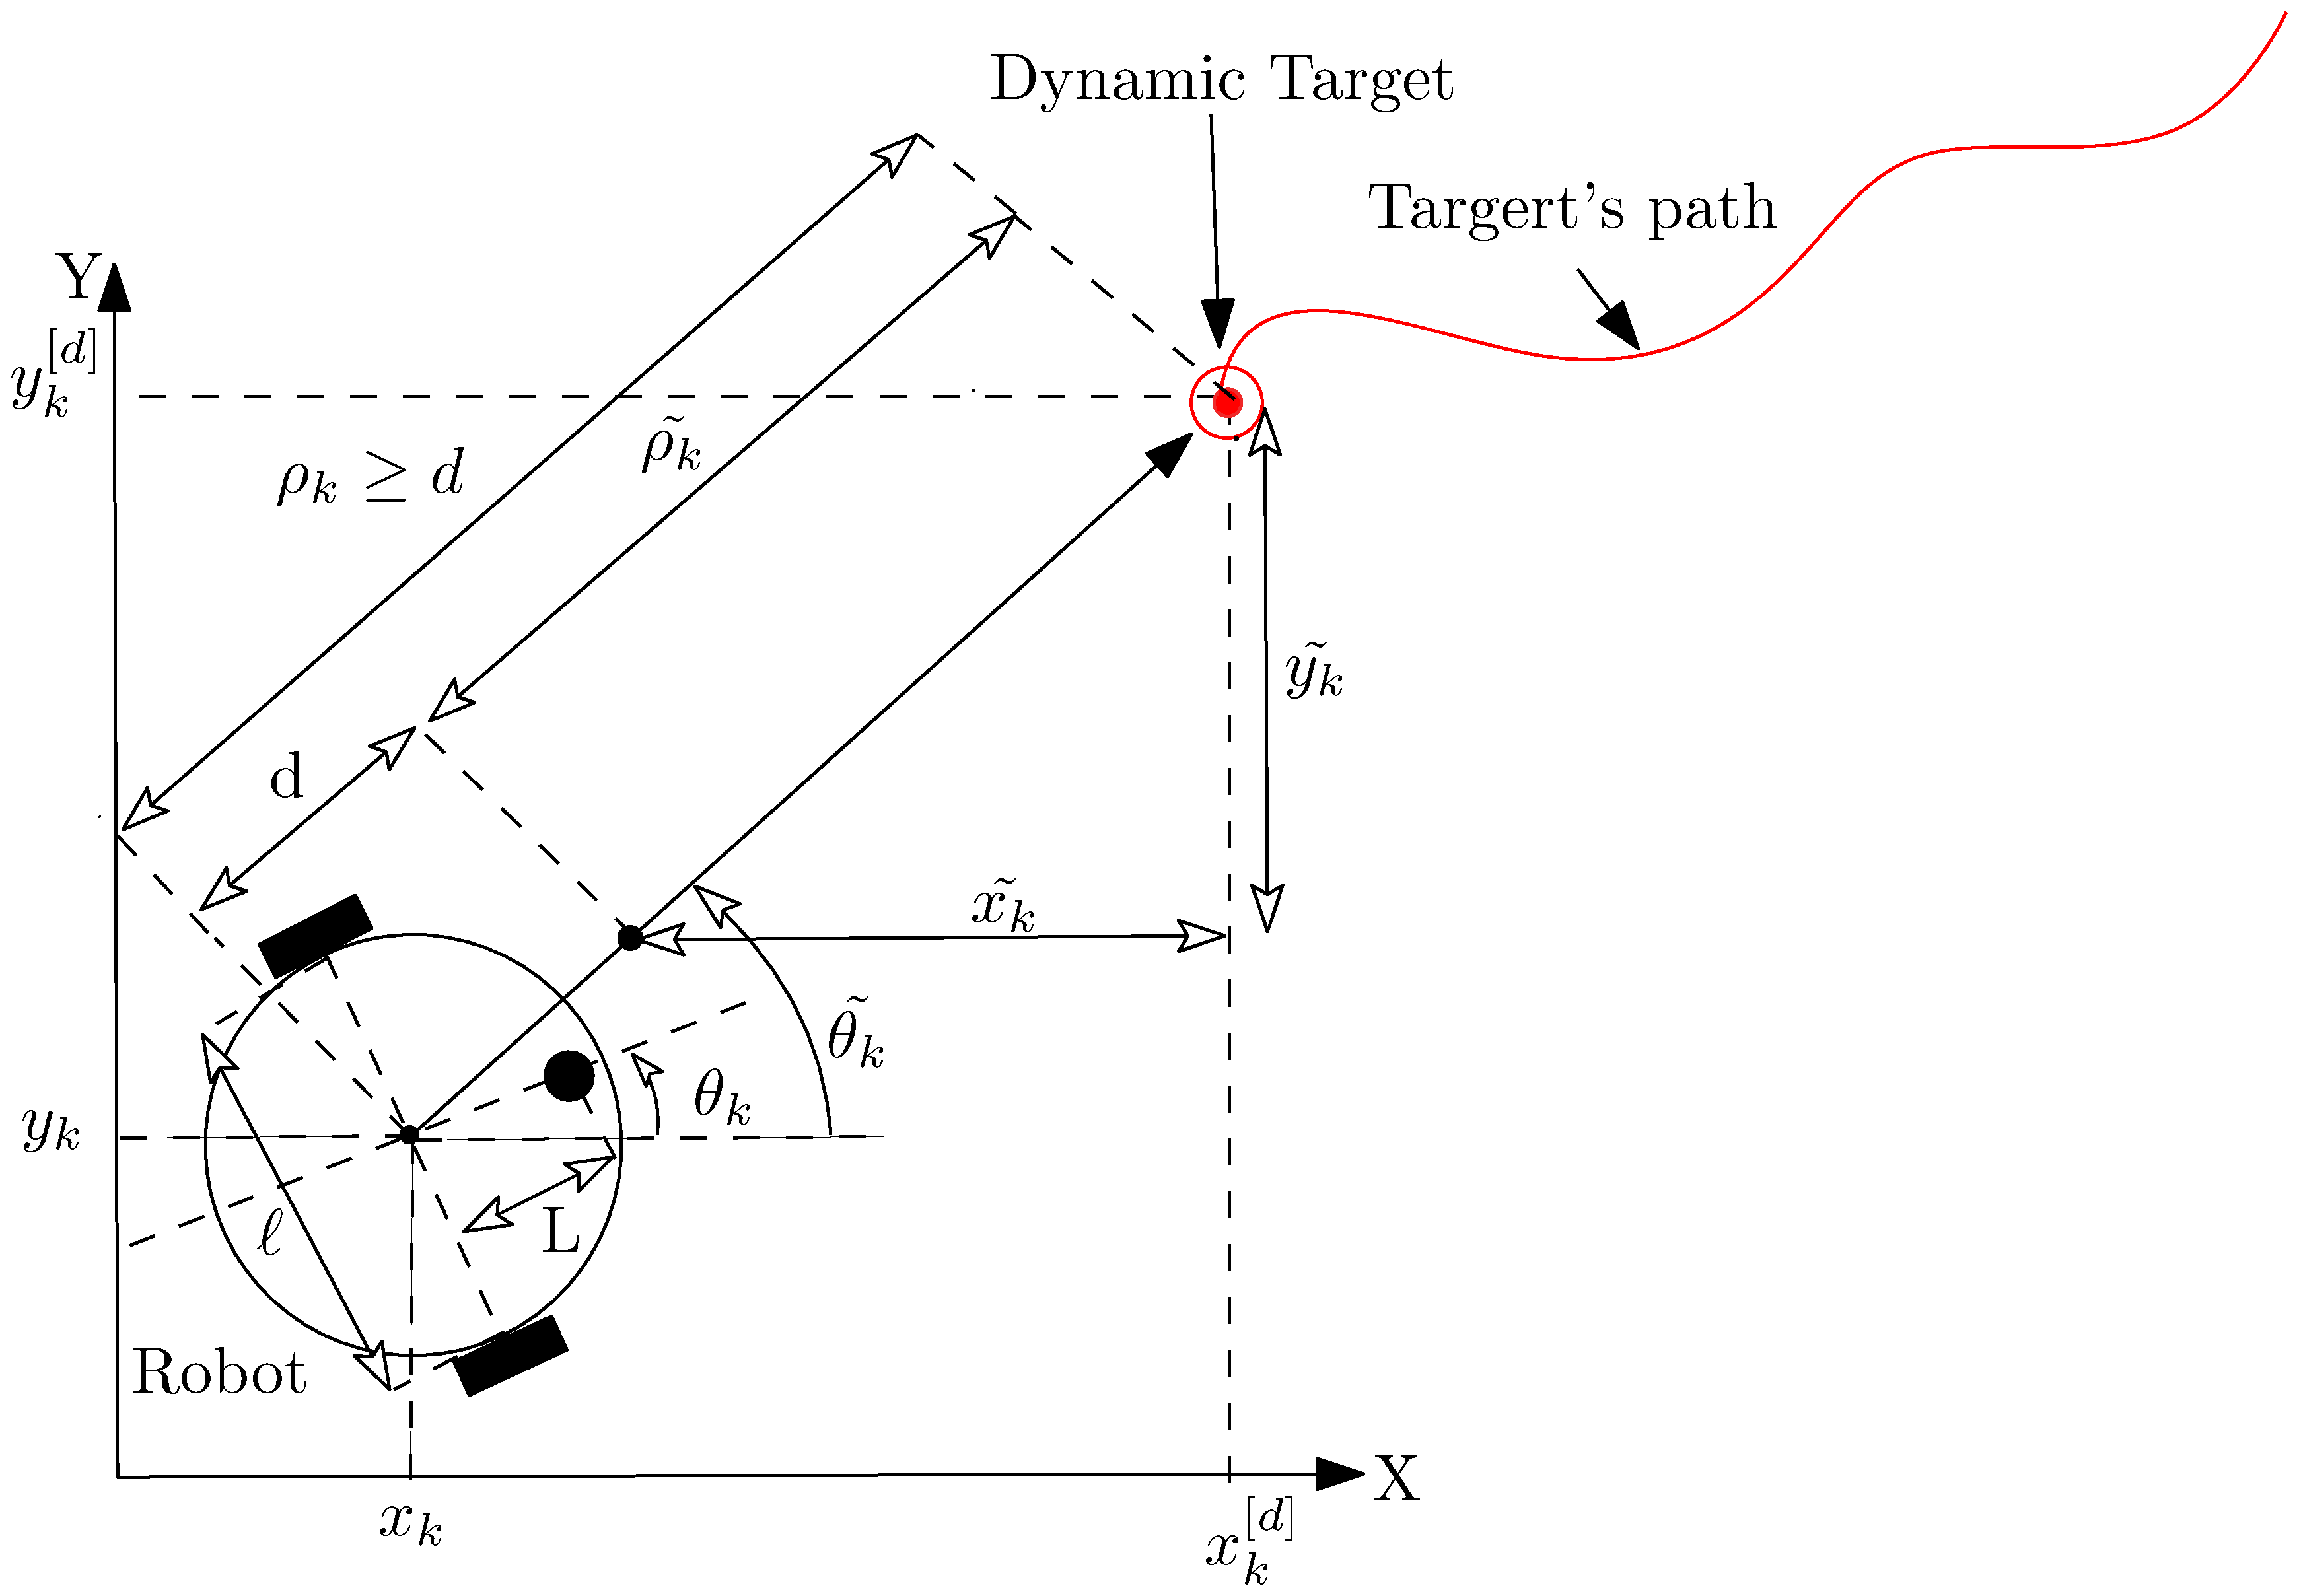
\includegraphics[width=0.45\textwidth]{figs/ipe/LFMICSetup.eps}
    }
   \caption{Mobile robot and its dynamic target tracking problem setup.}
   \label{fig:leaderFollowerSetup}
 \end{figure}
 \begin{subequations}
   \begin{align}
     \nu_{k} &= \frac{1}{2}(\nu_{R,k} + \nu_{L,k}),\\
     \omega_{k} &= \frac{1}{\ell}(\nu_{R,k} - \nu_{L,k}) = \frac{\nu_{k}}{L}\tan(\gamma_k) 	
   \end{align}
 \label{eq:robotModel1-DT}
 \end{subequations}
 %
 where $\omega_k = \frac{\nu_k}{L}\tan\gamma_k$ is the angular velocity of the robot's center $(x_k,y_k).$ Let us define the error vector as 
 \begin{align}
     \label{eq:stateError}
   \mathbf{e}_k = [\rho_k,\tilde\theta_k]^T=[\sqrt{\tilde{x}_k^2+\tilde{y}_k^2},\tilde{\theta_k}]^T% = \\
   % \begin{bmatrix}
   %   \sqrt{(x_k^{[d]} - x_k - d\cos\theta_k^{'})^2+
   %   (y_k^{[d]} - y_k - d\sin\theta_k^{'})^2},
   %   \theta_k^{'} - \theta_k
   % \end{bmatrix},
 \end{align}
% 
 where $\theta_k^{'} = \mathrm{atan2}\left(y_k^{[d]}-y_k, x_k^{[d]}-x_k\right)$
 and ${\rho_k} =\sqrt{\tilde{x}_k^2+\tilde{y}_k^2} $ is the Euclidean distance at time instant $k$ as shown in Fig.~\ref{fig:leaderFollowerSetup} with $\tilde{x}_k = x_k^{[d]} - x_k - d\cos\theta_k^{'},$ $\tilde{y}_k = y_k^{[d]} - y_k - d\sin\theta_k^{'},$ and $\tilde{\theta}_k = \theta_k^{'} - \theta_k.$ The control problem can then be formally stated as follows: Find $\nu_k$ and $\gamma_k$ such that ${\bf e}_k\to {\bf 0}$ as  $k\to\infty$ subject to~\eqref{eq:robotModelDT}~and~\eqref{eq:leaderDT}.

%
%
%  In the next section, a conventional trajectory tracking method is investigated to solve the problem~\eqref{eq:problem}. This is followed by the proposed approximate dynamic programming technique which is illustrated in section~\ref{sec:solutionADP}.




\section{Proposed actor-critic RL Approach}
\todo[inline]{Needs to be rewritten}

 \label{sec:RLSolution}

 The solution of the leader-follower formation problem is realized using a reinforcement learning approach. It employs model-free strategies for solving a temporal difference equation developed herein. This solution is equivalent to solving the underlying Bellman optimality equation for  the dynamical error model~\eqref{eq:stateError}. The relative importance of the states in the error vector ${\bf e}_k$ and the control decisions (linear velocity and steering angle) of the follower-robot are evaluated using the  performance (cost) index: %
 \begin{align}
 \label{eq:costFunctional}
 J = \sum_{k=0}^\infty \frac{1}{2}\left[{\bf e}_k^T \, {\bf Q} \, {\bf e}_k + {\bf u}_k^T \, {\bf R} \, {\bf u_k}\right],
 \end{align}    
 where ${\bf Q}\in\mathbb{R}^{2\times 2}$ and ${\bf R}\in\mathbb{R}^{2\times 2}$ are symmetric positive definite weighting matrices. The objective of the optimization problem, following~\cite{Lewis2013-Reinforcement}, is to find an optimal sequence of control polices $\{\mathbf{u}^*_k\}_{k=0}^\infty$ that minimizes the cost index $J$ along the state-trajectories~\eqref{eq:leaderDT}~and~\eqref{eq:robotModel1-DT}. Motivated by the structure of the convex quadratic cost functional~\eqref{eq:costFunctional}, let the solution of the tracking control problem employ the value function $V({\bf e}_k,{\bf u}_k)$ defined by %
 %
 \begin{equation*}
 \label{eq:valueFunction}
 V({\bf e}_k,{\bf u}_k) = \sum_{\kappa=k}^\infty \frac{1}{2}\left({\bf e}_\kappa^T\, {\bf Q}\, {\bf e}_\kappa + {\bf u}_\kappa^T \, {\bf R}\, {\bf u_\kappa}\right).
 \end{equation*}
 %
 This structure yields a temporal difference form (i.e., Bellman equation) as follows
 \begin{equation*}
 \label{eq:tempraldiffeq}
 V({\bf e}_k,{\bf u}_k)= \frac{1}{2}\left[{\bf e}_k^T\, {\bf Q}\, {\bf e}_k + {\bf u}_k^T\, {\bf R}\, {\bf u_k}\right] +V({\bf e}_{k+1},{\bf u}_{k+1}).
 \end{equation*}
 %
 Applying Bellman's optimality principle yields the optimal control policies ${\bf u}_k^*,~k\ge 0,$ such that~\cite{Lewis2012} %
 %
 \begin{align*}
 {\bf u}^*_k = \argmin_{{\bf u}_k}\left[\frac{1}{2}\left[{\bf e}^T_k\,  {\bf Q}\, {\bf e}_k +{\bf u}^T_k\,  {\bf R} \,  {\bf u}_k\right]   +
 V({\bf e}_{k+1},{\bf u}_{k+1})\right].
 \label{eq:argMinControlAction}
 \end{align*}
 %
 Alternatively, this optimal  policy form is equivalent to ${\bf u}^*_k = \argmin_{{\bf u}_k}\left[
 V({\bf e}_{k},{\bf u}_{k})\right].$
 Therefore, the underlying Bellman optimality equation follows %
 %
 \begin{equation*}
 \label{eq:BellOpt}
 V^*({\bf e}_k,{\bf u}^*_k)= \frac{1}{2}\left[{\bf e}_k^T\, {\bf Q}\, {\bf e}_k + {\bf u}_k^{*T}\, {\bf R}\, {\bf u}^*_k\right] +V^*({\bf e}_{k+1},{\bf u}^*_{k+1}),
 \end{equation*}
 %
 where $V^*(\cdot,\cdot)$ is the optimal solution for Bellman optimality equation. This temporal difference equation is utilized by reinforcement learning process which solves the following temporal difference approximation form %
 %
 \begin{align}
 \hat{V}(\mathbf{z}_k) = \frac{1}{2}\mathbf{z}_k^T\, \bar{\mathbf{P}}\, \mathbf{z}_k + \hat{V}(\mathbf{z}_{k+1}),
 \label{eq:valueFunctionEstimated}
 \end{align}
 %
 where $\mathbf{z}_k = \left[\mathbf{e}_k ,\mathbf{u}_k\right]^T\in\mathbb{R}^4,$ $V\left(\mathbf{e}_k,\mathbf{u}_k\right) \approx \hat{V}(\mathbf{z}_k),$  and $\bar{\mathbf{P}}$ is a symmetric block-diagonal matrix formed using $(\mathbf{Q},\mathbf{R}),$~\textit{i.e.,~}$\bar{\mathbf{P}} = \mathrm{blockdiag}(\mathbf{Q},\mathbf{R}).$ %
 The approximation of the solving value function $\hat{V}(\mathbf{z}_k)$ employs a quadratic form so that $\hat{V}(\mathbf{z}_k)=\frac{1}{2}\mathbf{z}_k^T\, \mathbf{P}\, \mathbf{z}_k,$ where $\mathbf{P}\in\mathbb{R}^{4\times 4}$ is a positive definite matrix. Hence, the optimal control strategy $\mathbf{u}_k^*$ can be expressed as follows %
 %
 \begin{align}
 \label{eq:modelFreePolicy}    
 \mathbf{u}_k^* = \argmin_{\mathbf{u}_k}\left[\hat{V}(\mathbf{z}_k)\right] = -\,  \mathbf{P}_{uu}^{-1}\, \mathbf{P}_{ue}\, \mathbf{e}_k,
 \end{align}
 %
 where $\mathbf{P}_{uu}$ and $\mathbf{P}_{ue}$ are sub-blocks of symmetric matrix $\mathbf{P}.$ %   
 %
 \todo[inline]{The following paragraph and the NN structure needs to be rewritten}
A two-step solution mechanism that is based on policy iteration is employed to solve the temporal difference equation~\eqref{eq:valueFunctionEstimated} using the policy~\eqref{eq:modelFreePolicy}. First, the adaptive critics are used to approximate the solving value function $\hat V(\cdot)$ using a multi-layer critic neural network as shown in Fig.~\ref{fig:nnCritic}. %
 
\begin{figure}
    \centering
    \fcolorbox{blue}{gray!5}{
        \begin{adjustbox}{max width = 0.45\textwidth}
            \tikzset{%
                input neuron/.style={
                    circle,
                    fill=green!50,
                    minimum size=0.7cm
                },
                neuron missing/.style={
                    draw=none, 
                    scale=1,
                    fill=white,
                    text height=0.01cm,
                    execute at begin node=\color{black}$\vdots$
                },
            }
           
            \tikzset{%
                hidden neuron/.style={
                    circle,
                    fill=blue!50,
                    minimum size=0.7cm
                },
                neuron missing/.style={
                    draw=none, 
                    scale=1,
                    fill=white,
                    text height=0.01cm,
                    execute at begin node=\color{black}$\vdots$
                },
            }
           
            \tikzset{%
                output neuron/.style={
                    circle,
                    fill=red!50,
                    minimum size=0.7cm
                },
                neuron missing/.style={
                    draw=none, 
                    scale=1,
                    fill=white,
                    text height=0.01cm,
                    execute at begin node=\color{black}$\vdots$
                },
            }
           
            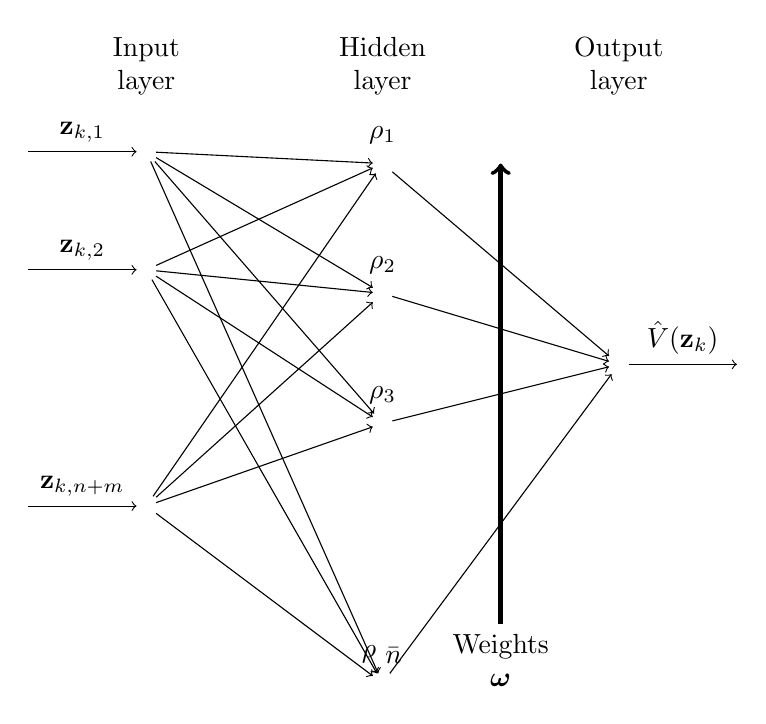
\begin{tikzpicture}[x=1.5cm, y=1.5cm]
           
            \foreach \m/\l [count=\y] in {1,2,missing,3}
            \node [input neuron/.try, neuron \m/.try] (input-\m) at (0,2.5-\y) {};
           
            \foreach \m [count=\y] in {1,2,3,missing,4}
            \node [hidden neuron/.try, neuron \m/.try ] (hidden-\m) at (2,2.5-\y*1.1) {};
           
            \foreach \m [count=\y] in {1}
            \node [output neuron/.try, neuron \m/.try] (output-\m) at (4,2.5-\y*2.8) {};
           
            \foreach \l [count=\i] in {1,2,n+m}
            \draw [<-] (input-\i) -- ++(-1,0)
            node [above, midway] {$\mathbf{z}_{k,\l}$};
           
            \foreach \l [count=\i] in {1,2,3,~\mbox{$\bar{n}$}}
            \node [above] at (hidden-\i.north) {$\rho_{\l}$};
           
            \foreach \l [count=\i] in {1}
            \draw [->] (output-\i) -- ++(1,0)
            node [above, midway] {$\hat{V}(\mathbf{z}_{k})$};
            % node [above, midway] {$\hat{V}_\l$};
           
            \foreach \i in {1,...,3}
            \foreach \j in {1,...,4}
            \draw [->] (input-\i) -- (hidden-\j);
           
            \foreach \i in {1,...,4}
            \foreach \j in {1}
            \draw [->] (hidden-\i) -- (output-\j);
           
           
           
            \foreach \l [count=\x from 0] in {Input, Hidden, Output}
            \node [align=center, above] at (\x*2,1.9) {\l \\ layer};
           
            \node [align=center, below] at (3,-2.5) {Weights \\ $\boldsymbol{\omega}$};
            \draw[->,ultra thick](3,-2.5) -- (3,1.4);
           
            \end{tikzpicture}
        \end{adjustbox}      
    }
    \caption{Critic neural network structure for approximating value function.}
    \label{fig:nnCritic}
      \end{figure}
 %      
 Second, the policy evaluation step of this process updates the critic weights $\bm{\omega}$ in real-time without acquiring any formation about the dynamics of the leader or follower dynamical systems  (the calculation mechanism of the critic weighs $\boldsymbol{\omega}$ is explained later on). This is done to search for a strictly better policy. %
 %

% Note that, the policy iteration computational setup rearranges the temporal difference expression~\eqref{eq:valueFunctionEstimated} such that %
 %
 \begin{equation}
 \label{eq:const}
 \mathbf{z}_k^T\, \mathbf{P}\, \mathbf{z}_k - \mathbf{z}_{k+1}^T\, \mathbf{P}\, \mathbf{z}_{k+1} = \mathbf{z}_k^T\, \bar{\mathbf{P}}\, \mathbf{z}_k. 
 \end{equation}
 %
 This equation is utilized repeatedly in order to evaluate a certain policy during at least $\eta\ge \bar n, \bar n= (2+2)(2+2+1)/2$ evaluation steps (i.e., the lowest evaluation interval spans $k$ to $k+\bar n$ calculation samples) in order to update the critic weights vector  $\boldsymbol{\omega}=\mathrm{vec}(\mathbf{P}),$ which consists of connection weights between the neurons of the hidden layer and the output layer of the critic neural network shown in Fig.~\eqref{fig:nnCritic}. The operator $\mathrm{vec}(\mathbf{P})$ forms the columns of the $\mathbf{P}$ matrix into a column vector $\mathbf{\omega}$ of dimension $\bar{n}=15$ since the matrix $\mathbf{P}$ is a symmetric matrix. The left hand side of~\eqref{eq:const} is expressed using the following critic approximation form %
 %
 $$\hat{V}(\mathbf{z}_k)-\hat{V}(\mathbf{z}_{k+1})=\boldsymbol{\omega}^T\tilde{\bm{\rho}}(\mathbf{z}_{k,k+1}),$$
 %
 where $\tilde{\bm{\rho}}(\mathbf{z}_{k,k+1})=\bm{\rho}(\mathbf{z}_k)-\bm{\rho}(\mathbf{z}_{k+1}) \in \mathbb{R}^{10 \times 1}, \, \bm{\rho}(\mathbf{z}_k)=\left(\mathbf{z}^q_k\otimes\mathbf{z}^h_k\right)$ $(q=1,\dots, 5, \,\, h=q,\dots,5),$ and $\boldsymbol{\omega}^T = [0.5 \, P^{11},P^{12},P^{13},P^{14},  \, 0.5 \, P^{22}, P^{23},P^{24},$ $\,0.5 \, P^{33}, P^{34},\,0.5 \ P^{44}, ]^T \in \mathbb{R}^{1\times 15}$ ($P^{ij}$ is the $ij^{th}$ entry of matrix $\mathbf{P}$). %
 %
 The critic weights $\boldsymbol{\omega}$ are updated using a gradient descent approach, where the tuning error $\varepsilon_k$ at each computational instance $k$ follows $\varepsilon_k =\boldsymbol{\omega}^T\tilde{\bm{\rho}}(\mathbf{z}_{k,k+1})-{v}_k,$ where $v_\kappa = \frac{1}{2}\mathbf{z}_{k}^T \, \bar{\mathbf{P}} \, \mathbf{z}_{k}$. As detailed earlier, it is required to perform at least $\eta \ge \bar n$ evaluation steps before updating the critic weights $\boldsymbol{\omega}$ (i.e., finding the new improved policy). Hence, it is required to minimize the sum of square errors such that %
 %
 \begin{multline*}
   \delta_c =\sum_{\kappa=0}^{\eta-1}\frac{1}{2}(\boldsymbol{\omega}^T\tilde{\bm{\rho}}(\mathbf{z}_{k+\kappa,k+\kappa+1})-{v}_{k+\kappa})^2 = \frac{1}{2}\| \mathbf{v} - \bm{\Lambda}\bm{\omega}\|^2\\
   =\frac{1}{2}\left(\mathbf{v} - \bm{\Lambda}\bm{\omega}\right)^T \left(\mathbf{v} - \bm{\Lambda}\bm{\omega}\right), 
 \end{multline*}
 where $\bm{\Lambda} = [{\bf o}_0,{\bf o}_1,\ldots,{\bf o}_{\eta-1}]^T \in \mathbb{R}^{\eta\times 10}$ with ${\bf o}_\kappa = \tilde{\bm{\rho}}^T({\bf z}_{k+\kappa, k+\kappa+1}) \in \mathbb{R}^{1\times 15}$ and ${\bf v} =[v_0,v_1,\ldots,v_{\eta-1}]^T \in \mathbb{R}^{\eta}$ with $v_\kappa = \frac{1}{2}\mathbf{z}_{k+\kappa}^T \, \bar{\mathbf{P}} \, \mathbf{z}_{k+\kappa}$ for $\kappa = 0,1,\ldots, \eta-1$. %
 Therefore, the update law of the critic weights using the gradient decent approach for at least $\bar n$ samples is given by %
 \begin{multline}
   \bm{\omega}^{[r+1]} = \bm{\omega}^{[r]} - \ell_c\frac{\partial\delta_c}{\partial \bm{\omega}} = \bm{\omega}^{[r]} - \ell_c\left(-\bm{\Lambda}^T\mathbf{v} + \bm{\Lambda}^T \bm{\Lambda}\bm{\omega}^{[r]}\right)\\ 
 =\bm{\omega}^{[r]} - \ell_c \bm{\Lambda}^T\left(\bm{\Lambda}\bm{\omega}^{[r]}-\mathbf{v}\right), 
 \label{eq:criticWeights}
 \end{multline}
 %
 where $0<\ell_c<1$ is a critic learning rate and $r$ is the  update index of the critic weights. 

% The newly computed critic weights $\boldsymbol{\omega}$ are used to reconstruct the matrix ${\bf P}$ (i.e., updating the solving value function and hence calculating the associated policy) such that 
 %
 \begin{center}
 ${\bf P}=\begin{bmatrix} 
 2\,\omega^{1}    & \omega^{2}      & \omega^{3}       & \omega^{4}        \\ 
 \omega^{2}       &2\, \omega^{5}   & \omega^{6}       & \omega^{7}        \\
 \omega^{3}       & \omega^{6}      &2\, \omega^{8}   & \omega^{9}   \\   
 \omega^{4}       & \omega^{7}      & \omega^{9}      & 2\,\omega^{10}      
 \end{bmatrix}\in \mathbb{R}^{4\times 4},$
 \end{center}
 %
 where $\omega^{i}$ is the $i^{th}$ entry of the weight vector $\bm{\omega}.$ 
 \todo[inline]{merge the actor weights discussion with the rest}
 The critic wegihts are then used to update the actor weights which maps the state error to the desired ploicy (control actions) at every time step $t$ with the following equation:
 \begin{align}
 \label{eq:actorWeightsPolicy}    
 \mathbf{u}_k  =  \mathbf{\omega_a^{T}} \mathbf{e}_k
 \end{align}   
 Applying a similar gradient descent approach as with the critic weights the actor weights are updated as follows:
\begin{align}
   \bm{\omega_a}^{[r+1]} = \bm{\omega}^{[r]} - \ell_a(\mathbf{u}_k-\mathbf{u}_k^*)\mathbf{e}_k, 
 \label{eq:actorWeights}
 \end{align}
 where $\ell$ is the actor learning rate. 
 \\
 The complete policy iteration solution process for the leader-follower problem is detailed out in Algorithm \ref{alg:ModelFreeTracking}. %
 %
 \begin{algorithm2e}{
     \caption{\label{alg:ModelFreeTracking} Model-free actor-critic reinforcement learning using the policy iteration solution.}
     \DontPrintSemicolon
     \KwIn{Sampling-time $T_s,$ $\mathbf{Q},~\text{and}~\mathbf{R}$ }
     \KwOut{Error trajectory $\mathbf{e}_k,$ for $k=0,1,\ldots$}
     % \KwData{Map representation using occupancy grid technique}
     % \KwResult{output******************************}
     \Begin{
         $k=0, r = 0$ \tcc*[h]{Discrete time and policy indices}\;
         $\eta = (n+m)(n+m+1)/2$\;
         Initialize $\mathbf{P}^{[0]}$ \tcc*[h]{Positive definite}\;
                 Set offset distance $d$\;
                 Given approximate initial poses of leader and follower, compute $\mathbf{e}_0$ using error model~\eqref{eq:stateError}\;
                 Compute follower's input $\mathbf{u}_0^{[0]}$ using policy~\eqref{eq:actorWeightsPolicy}\;
         \Repeat(\tcc*[h]{Main timing loop}){Tracking errors are zero}
         {
             Find $\mathbf{e}_{k+1}$ using~\eqref{eq:stateError}\;
             Compute policy $\mathbf{u}_{k+1}^{[r]}$ using~\eqref{eq:actorWeightsPolicy}\;
             %Evaluate and record Equation~\eqref{eq:modelFreeMatrixSolution}\;
             \If{[$(k+1)~\mathrm{modulo}~\eta]==0$ }
             {
                 $r\leftarrow r+1$\tcc*[h]{Evaluate policy}using~\eqref{eq:modelFreePolicy}\;
                 Solve for the critic-weights $\bm{\omega_c}$ using~\eqref{eq:criticWeights}eights}\;
                 Solve for the actor-weights $\bm{\omega_a}$ using ~\eqref{eq:actorWeights}\;\;
                 Construct matrix $\mathbf{P}^{[r]}$ using vector $\bm{\omega_c}$\;
 %                \eIf{$\|\mathbf{P}^{[r]} - \mathbf{P}^{[r+1]}\|<\varepsilon$}{Set $\mathbf{u}_{k+1}^*\leftarrow\mathbf{u}_{k+1}^{[r]}$}{$k\leftarrow k+1$ }
             }
 %        {
 %                $k\leftarrow k+1$
 %            }
         $k\leftarrow k+1$
         }
     }
 \end{algorithm2e}    
    
    


  

 \section{Computer Experiments and Results}
 \label{sec:resultsExperiments}
 \todo[inline]{review}
 This section adopts the theoritical results discussed in the previous section by simulating the Algorithm using the Pioneer 3-DX  robot. The proposed Actor-Critic RL algorithm is tested using the commercial robot simulator CoppeliaSim in integration with Matlab software as a prelminary step to implement the Algorithm experimantally in real world.Here we present the performance of the proposed method and the convergence characterisitcs of the actor and critic weights. The weighting matrices are set to $\mathbf{Q} = \mathrm{diag}[0.001,0.001]$ and $\mathbf{R} = \mathrm{diag}[10^{-5}, 10^{-5}].$ % 
  \[Q=0.001 
  \begin{bmatrix}
  1       & 0   \\
  0       & 1   \\
  \end{bmatrix},
  R=0.00001
  \begin{bmatrix}
  1       & 0 \\
  0       & 1 
  \end{bmatrix}.\]
  
  
 The actor and critic learning rates $\ell_c$,$\ell_a$ are set to  $0.0001$ and $0.01$ respectively. The sampling time $T_s$ is set to $0.001 \sec.$ The desired distance offset between the leader and the follower is set to $ d = 0.2$ [m].

 
  During the simulation CoppeliaSim simulator accuratly mimics what would happen in a realworld scenario following idustry standatrds and guidlines.The setup of the virtual expirement is illustrated  in figure \ref{fig:CoppeliaSim Scene} where pioneer robot model was initally placed at position $(x,y) = (-1,-2.5) $ [m] with an orientation $\theta = 0 \degree$ .The Target which is modeled as a cylinder object was initially located at a random position around  $(x,y) = (0,0)$ [m]. The simulation was run for the duration of 15 seconds. 
  The Target is set to move on a completely random trajectory starting from a random position. We intensify that the follower robot has no previous knoweledge of the dynamic model of the moving target nor it's initial position. The results obtained by the simulation are shown in figure \ref{fig:simulationResults}. the control actions of the pioneer robot are determined by the random actor weights .we clearly see tracking error converges to the desired value of $d$ = 0.2 [m] along with control signal converging to values that allows target tracking. the results reveal the ability of the proposed algorithm to sucessfully track the dynamic moving target and adapt to the changes in the target's path in an online manner.      
\begin{figure}
   \centering
   \fcolorbox{gray!10}{gray!5}{
     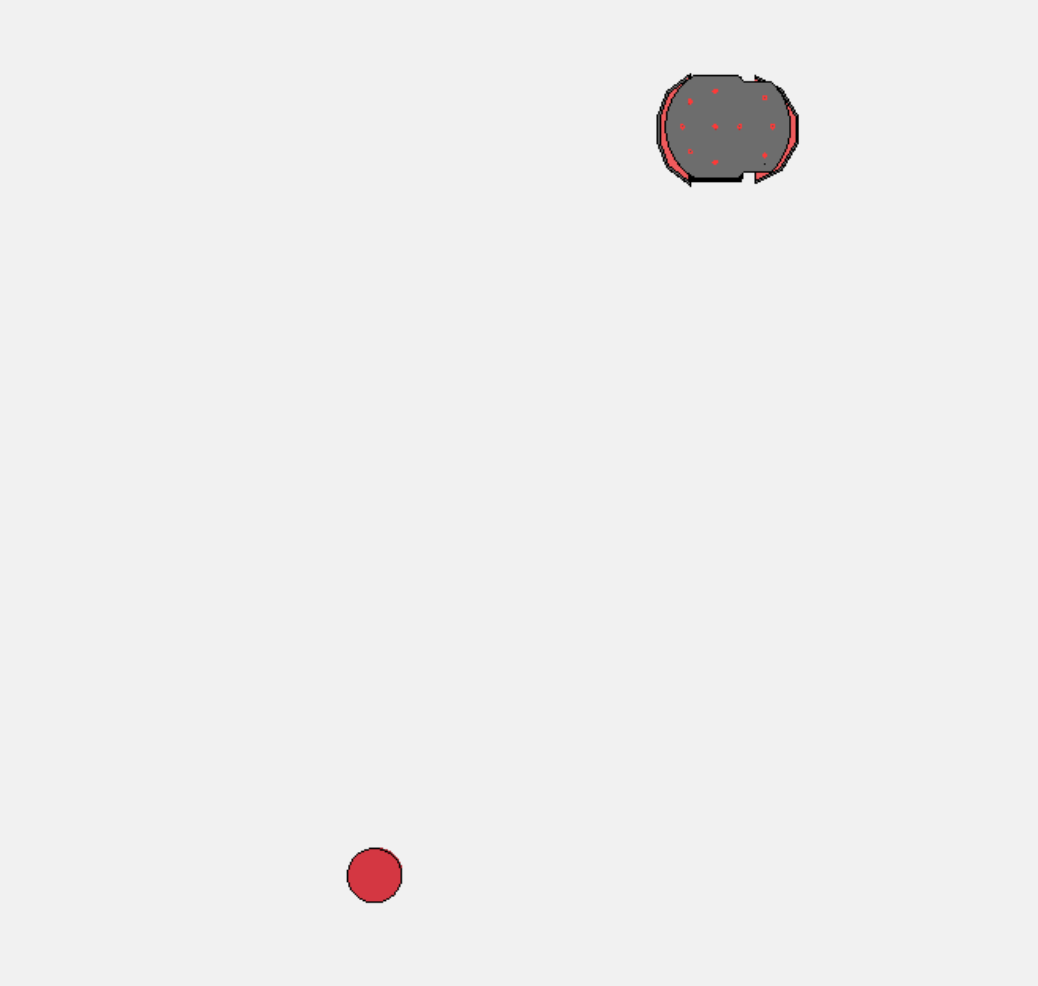
\includegraphics[width=0.45\textwidth]{figs/coppeliasim.png}
`     }
   \caption{Simulation Setup}
   \label{fig:CoppeliaSim Scene}
 \end{figure}  
    
 \begin{figure*}[htbp]%
 
 \subfigure[][]{%
    \label{fig:trajectoryRandom}%
    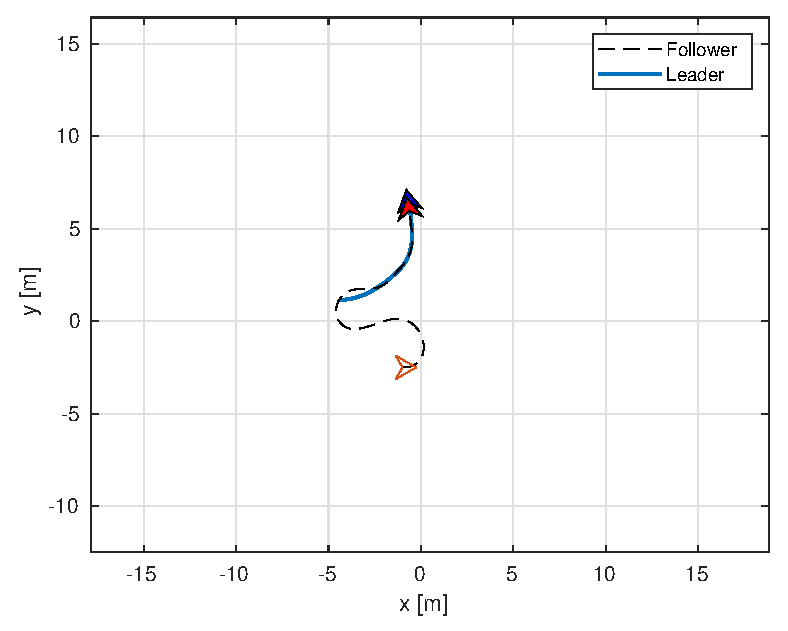
\includegraphics[width=0.48\textwidth,height=0.25\textheight]{figs/coppelia/firstScenario/trajectoryRandomPathDistance.eps} }
	\subfigure[][]{%    
    \label{fig:euclideanDistance}%
    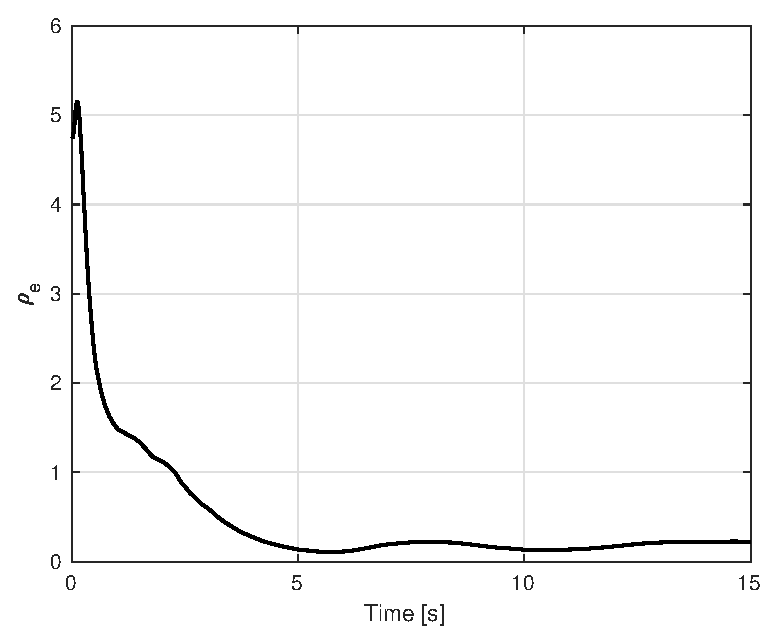
\includegraphics[width=0.48\textwidth,height=0.25\textheight]{figs/coppelia/firstScenario/euclideanDistance.eps} }
\subfigure[][]{%
    \label{fig:stateErrorRandom}%
    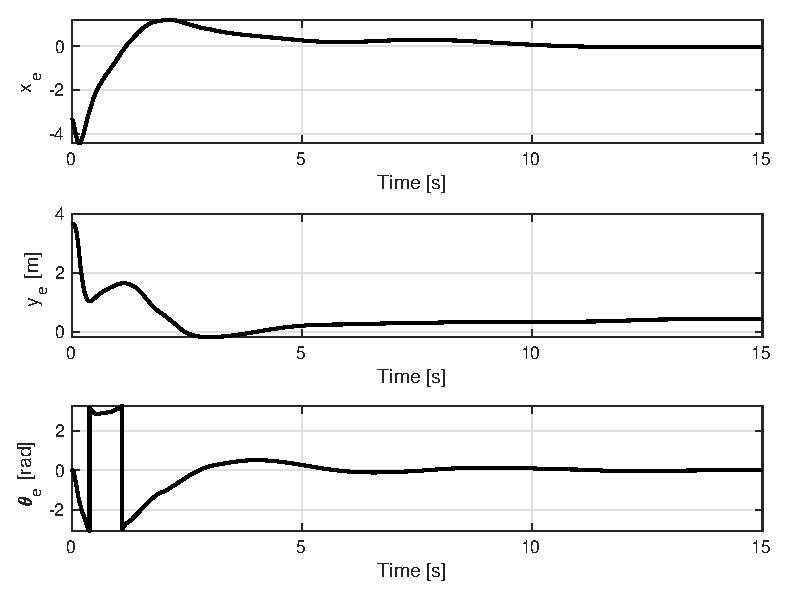
\includegraphics[width=0.48\textwidth,height=0.25\textheight]{figs/coppelia/firstScenario/stateErrorRandomPathDistance.eps} }
 \subfigure[][]{%
    \label{fig:controlInputsRandom}%
    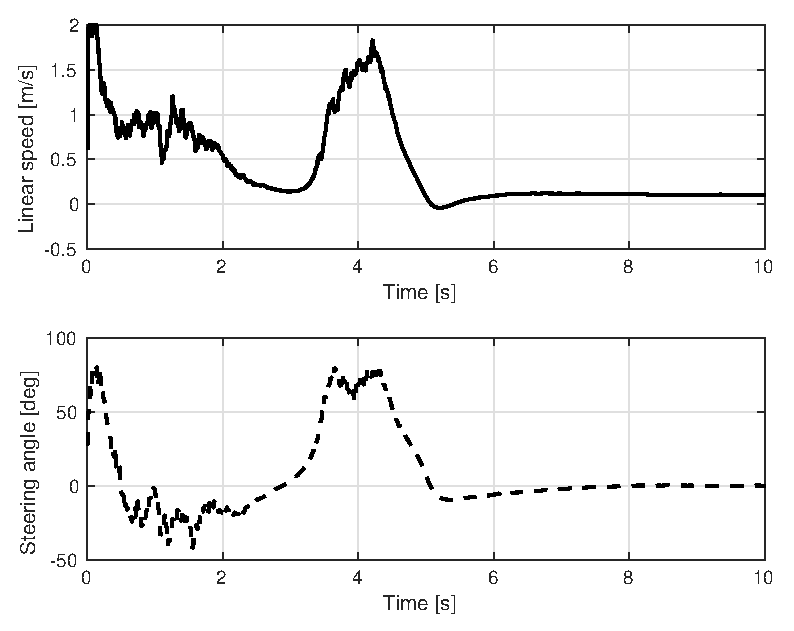
\includegraphics[width=0.48\textwidth,height=0.25\textheight]{figs/coppelia/firstScenario/controlInputRandomPathDistance.eps} }
 \subfigure[][]{%
    \label{fig:weightRandomDistance}%
    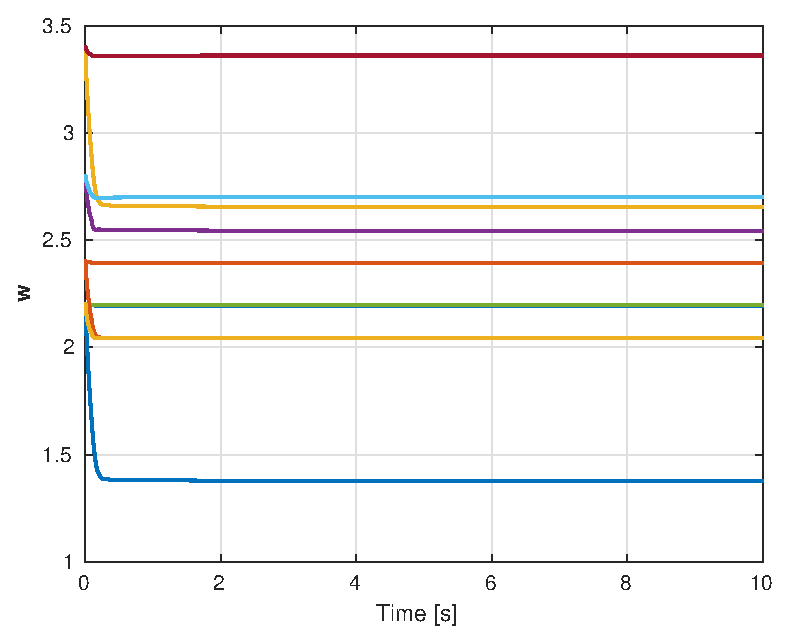
\includegraphics[width=0.48\textwidth,height=0.25\textheight]{figs/coppelia/firstScenario/weightRandomPathDistance.eps} }
     \subfigure[][]{%
    \label{fig:actorWeightRandomDistance}%
    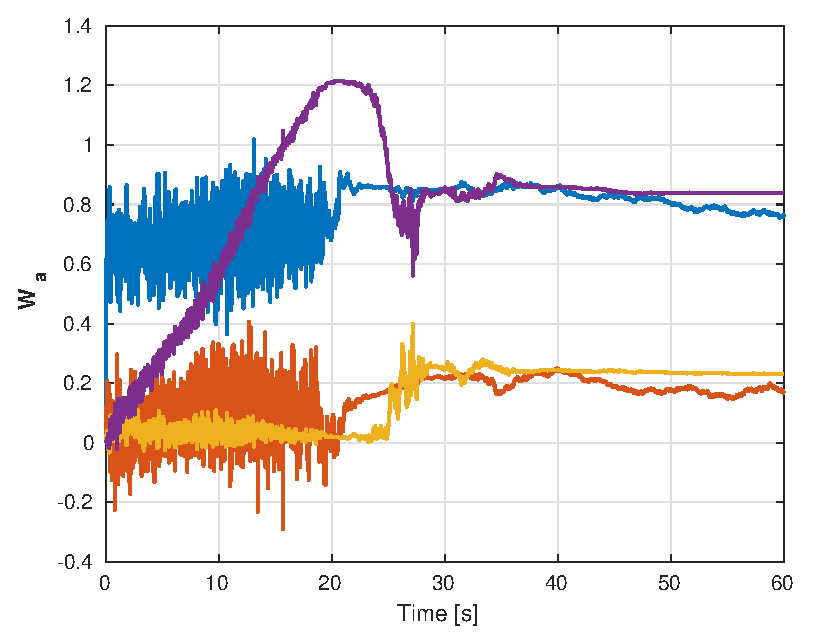
\includegraphics[width=0.48\textwidth,height=0.25\textheight]{figs/coppelia/firstScenario/weightActor.eps} }
\caption[Leader-follower performance for random trajectory.]{Performance in tracking random trajectory: 
  \subref{fig:trajectoryRandom} leader-follower trajectories,~\subref{fig:stateErrorRandom} state error,~\subref{fig:controlInputsRandom} linear speed and steering angle of the follower; and    \subref{fig:weightRandomDistance} learning weights.}%
  \label{fig:peformanceRandomTrajectory}%
	\label{fig:simulationResults}
\end{figure*}


 \section{Conclusion} \label{sec:conclusion}
	\todo[inline]{review}
	A model free actor-critic reinfoncement learning algorithm for dynamic target tracking has been validated using virtual robot experimantation platform where a differenitial drive mobile robot and a randomly moving target are utilized in the simulation.Opposed to previous approaches in the litrature this Algorithm possess the advantage of being completlety model free and doesn't rely on any dynamic model to be known in priori. The actor weights which drives the control actions of the robot sucessfully converge to values that enable the robot to track the moving target through unplanned trajectory. To the authors knowlege this work is the first of its kind to employ a model-free actor-critic RL approach  in the context of dynamic target tracking. In future work the proposed approach will be applied to multi-robot scenarios where a number of robots are to achieve a certain task in unknown enviroments.          
 


	\bibliographystyle{IEEEtran}
\bibliography{bib/refsSuruzWeb,bib/refsMultiAgent,bib/refsRoboticsJournals,bib/refsRoboticsConferences,bib/refsGenericControl,bib/refsBooksTRTheses,bib/refsReinforcementLearningADP,bib/refsRL-Keshtkar}
\end{document}

%%% Local Variables:
%%% mode: latex
%%% TeX-master: t
%%% End:
